\section{Overview of a Search Engine}\label{sec:overview}

In this section, we give a brief description of the workflow and evaluation of a search engine.
A search engine typically consists of two processes, i.e., indexing process and matching process~\cite{V99}.
Indexing is the process of selecting terms to represent a text.
Matching is the process of applying a retrieval model to feed back relevant documents.
Fig.~\ref{fig:frame} shows the general workflow of an engine to search for the information need in a collection of material.
\begin{figure}
  \centering
  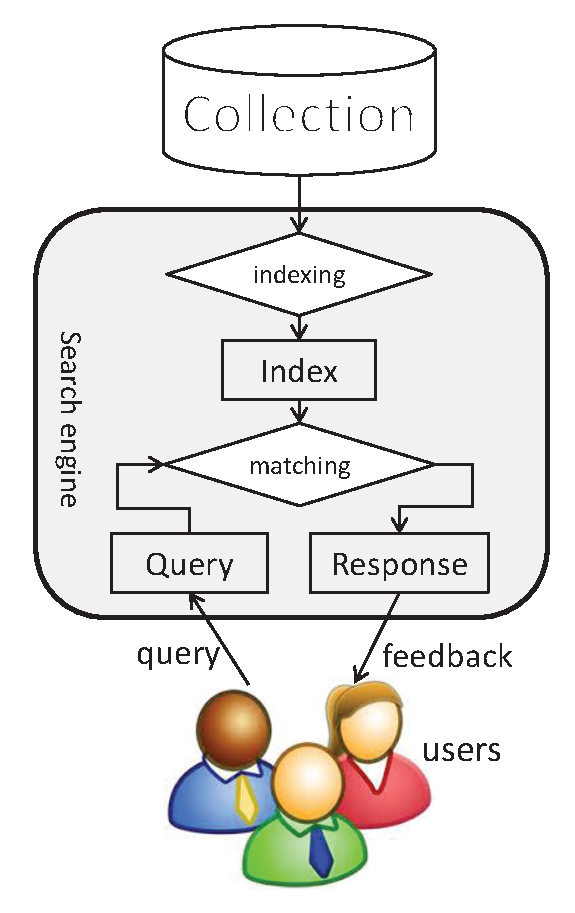
\includegraphics[width=.5\columnwidth]{frame1}
  \caption{The framework of a search engine.}\label{fig:frame}
\end{figure}

\subsection{Indexing}

In order to be searchable, the dataset should firstly be indexed and stored.
A general indexing process usually contains following steps.
\begin{enumerate}
  \item \textbf{Tokenization}. Break apart the components (e.g., words) of a document.
  \item \textbf{Removal of stop words}. Remove frequently used words such as prepositions and pronouns.
  \item \textbf{Stemming}. Conflate related word forms to a common stem by removing suffixes.
  \item \textbf{Index construction}. Build an appropriate index for the system to further search.
\end{enumerate}

The main step is to build an appropriate search index. It can provide the results for queries.
Without a search engine index, the search engine would take considerable
amounts of time and effort each time a search query is initiated.
There are two main parts in a search engine index, i.e., design factors and data structures.
The design factors of a search engine index outline the architecture of the index and decide how the index actually works, such as merge factors, index size, storage techniques, and so on.
The data structures of a search engine index can be forward index, inverted index, document-term matrix, and so on.

\subsection{Retrieval models}

After obtaining the search engine index, a proper retrieval model is applied to find the relevant documents and their rankings. There are many retrieval models available.

%The simplest IR model is the Boolean model. In this model, the index is a document-term matrix. The queries are represented as Boolean combinations of terms, and the set of documents that satisfied the Boolean expression was retrieved in response to the query. We only need to consider whether a term is in a document or not, without counting the frequency of each term in a document.  Moreover, we cannot rank the returned results.

The vector space model is a commonly used retrieval model.
It casts queries and documents as finite dimensional vectors, where each element is the weight of a term in a document computed using numerous variations of TF-IDF. To compute a score between a document and a query, the model needs to measure the similarity between the query and document vectors, such as using cosine function. Thus, the main task is to construct a proper term weight scheme.
A basic TF-IDF weighting scheme can be described as follows~\cite{MRS08}.
Suppose $C$ is a document collection with $N$ documents, $d$ is a document, and $t$ is a term.
The term frequency (TF) of $t$ in $d$, denoted as $tf_{t,d}$, is defined as the number of occurrences of term $t$ in document $d$.
The document frequency of $t$, denoted as $df_t$, is the number of documents that contain $t$ in the collection $C$, and the inverse document frequency (IDF) is defined as $idf_t=\frac{N}{df_t}$.
Thus, the final term weighting of $t$ in $d$ can be described as:
\begin{equation}
	  w_{t,d}=\left\{
  \begin{array}{ll}
    (1+\log_{10}tf_{t,d})\times \log_{10}\frac{N}{df_t}, & tf_{t,d}>0 \wedge df_{t}>0\\
    0, & tf_{t,d}\cdot df_{t}=0
  \end{array}\right.
\end{equation}
The final score for document $d$ corresponding to query $q$ can be measured by the summation of the weights of matched terms (Eq. \ref{eq:sum}),  or the cosine similarity (Eq. \ref{eq:cos}).
\begin{equation}\label{eq:sum}
  score(q,d)=\sum_{t\in q\cap d}w_{t,d}
\end{equation}
\begin{equation}\label{eq:cos}
  cos(\vec{q},\vec{d})=\frac{\vec{q}\cdot \vec{d}}{\|\vec{q}\|\|\vec{d}\|}=\frac{\sum_{i=1}^{|V|} q_id_i}{\sqrt{\sum_{i=1}^{|V|} q_i^2}\sqrt{\sum_{i=1}^{|V|} d_i^2}}
\end{equation}
where $\vec{q}$ and $\vec{d}$ are the weighted vectors whose elements are the weights of the collection's terms in $q$ and $d$, respectively; $q_i$ and $d_i$ are the term weight of term $i$ in $q$ and $d$, respectively; and $|V|$ is the number of terms in collection $C$.


%Note that in \emph{Lucene}, the scoring function is defined as
%\begin{equation}\label{lucenescore}
%  score(q,d)=coord(q,d)\cdot queryNorm(q) \cdot (\sum_{t\in q} (tfw_{t,d} \cdot idf_t^2 \cdot t.))
%\end{equation}
%the TF weight of a term $t$ in document $d$, denoted as $tfw_{t,d}$, is defined as $tfw_{t,d}=\sqrt{tf_{t,d}}$, and the IDF weight of a term $t$ in document $d$ is defined as $idfw_t=1+\frac{N}{df_{t}+1}$.


The probabilistic models are also widely used. The key part of the probabilistic models is to estimate the probability of relevance of the documents for a query. This is where most probabilistic models differ from one another~\cite{paik13}. Among the existing probabilistic models, BM25~\cite{JWR1,JWR2} is one of the most widely used and robust retrieval models. For simplicity, we only give some forms that build up to the standard form now used for document scoring. The simplest score for document $d$ facing query $q$ is just idf weighting of the query terms, i.e.,
\begin{equation}\label{eq:BM25_1}
  score(q,d)=\sum_{t\in q} \log{\frac{N}{df_t}}
\end{equation}

An improvement on Eq. \ref{eq:BM25_1} by factoring in the frequency of each term and document length can be described as:
\begin{equation}
  score(q,d)=\sum_{q \in d} \log{[\frac{N}{df_t}]}\times  \frac{(k_1+1)tf_{t,d}}{k_1((1-b)+b\!\times\! \frac{L_d}{L_{ave}})+tf_{t,d}}
\end{equation}
where $L_d$ and $L_{ave}$ are the length of document $d$ and the average document length for the whole collection respectively.
$k_1$ and $b$ are the positive tuning parameters that calibrate the term frequency scaling and document length scaling.

If the query is long, we might also use similar weighting for query terms. Thus, the improved formula can be described as follows.
\begin{flalign}
  {score(q,d)}=&\sum_{q \in d} \{ \log{[\frac{N}{df_t}]}
  \!\times\!\frac{(k_1+1)tf_{t,d}}{k_1((1-b)+b\!\times\! \frac{L_d}{L_{ave}})+tf_{t,d}} &&\nonumber\\
  &\!\times\! \frac{(k_3+1)tf_{t,q}}{k_3+tf_{t,q}} \}&&
\end{flalign}

At last, we give a brief description of the \emph{Lucene's Conceptual scoring formula} and \emph{Lucene's Practical Scoring Function}.
The detailed description can be found in~\cite{sim}.
First, the \emph{Lucene's Conceptual scoring formula} for a single field in the index is defined as follows.
\begin{flalign}
  {score(q,d)}=&Coord(q,d)\!\times\! QueryBoost(q)
    \!\times\! \frac{\vec{q}\!\times\! \vec{d}}{\|\vec{q}\|} \nonumber\\
    &\!\times\! DocLenNorm(d)\!\times\! DocBoost(d)
\end{flalign}
where
$Coord(q,d)$ is a score factor based on the fraction of the query terms in document $d$;
$QueryBoost(q)$ is the users specifying boosts to query $q$, and it is known when search starts;
$DocLenNorm(d)$ is a different document length normalization factor, which normalizes to a vector equal to or larger than the unit vector; and
$DocBoost(d)$ is the a document boost given by users, and it specifies the importance of $d$ relative to other documents.
Second, the \emph{Lucene's Practical Scoring Function} further consider the search time of each term in the query. The computational formula can be described as follows.
\begin{flalign}
  score&(q,d)=Coord(q,d)\!\times\! QueryNorm(q) \nonumber\\
    &\!\times\! \sum_{t\in q} (tf(t,d)\!\times\! idf(t)\!\times\! t.getBoost()\!\times\! norm(t,d))
\end{flalign}
where
$tf(t,d)=\sqrt{tf_{t,d}}$, and $idf(t)=1+\frac{N}{df_{t}+1}$;
$t.getBoost()$ is a search time boost of term $t$ in the query $q$;
the factor $norm(t,d)$ considers the document boost, field boost, and length norm.
$QueryNorm(q)$ is a normalizing factor used to make scores between queries comparable, and it does not affect document ranking.

%Based on the knowledge described in this section, we give the detailed implementation of a search engine and two further applications in the following two sections.

\subsection{Evaluation of a Search Engine}

When a search engine is developed, we must to measure its effectiveness.
The standard approach to information retrieval system evaluation revolves around the notion of relevant and non-relevant documents.
Note that relevance is assessed relative to an information need, not a query.
Two most frequent and basic measures are \emph{precision} and \emph{recall}.
Precision, denoted as $P$, is the fraction of retrieved documents that are relevant.
%\begin{equation}
%  P=\frac{\text{\# of relevant items retrieved}}{\text{\# of retrieved items in the collection}}
%\end{equation}
Recall, denoted as $R$, is the fraction of relevant documents that are retrieved.
%\begin{equation}
%  R=\frac{\text{\# of relevant items retrieved}}{\text{\# of relevant items in the collection}}
%\end{equation}
Considering the contingency table shown in Table \ref{tbl:contingency}, we have:
\begin{table}
\centering
\caption{\small{Contingency Table of Relevance and Retrieval}}\label{tbl:contingency}
  \begin{tabular}{|c|c|c|}
             \hline
             % after \\: \hline or \cline{col1-col2} \cline{col3-col4} ...
             & Relevant & Non-Relevant  \\
             \hline
             Retrieved & $tp$ & $fp$ \\
             \hline
             Not Retrieved & $fn$ & $tn$ \\
             \hline
  \end{tabular}
\end{table}
\begin{equation}\label{eq:p_r}
  P = \frac{tp}{tp+fp},\quad  R = \frac{tp}{tp+fn}
\end{equation}
where $tp$, $fp$, $fn$, and $tn$ are the numbers of items that are relevant and retrieved, non-relevant but retrieved, relevant but not retrieved, and non-relevant and not retrieved.
Then, the accuracy of an IR system can be measured as $accuracy=\frac{tp+tn}{tp+fp+fn+tn}$.

The advantage of having the two numbers for precision and recall is that one is more important than the other in many circumstances.
However, the two quantities clearly trade off against one another.
A single measure to compute the trade-off between precision and recall is the $F$-measure. It is the weighted harmonic mean of precision and recall, i.e.,
\begin{equation}\label{eq:F}
  F_{\beta}=\frac{1}{\alpha \frac{1}{P}+(1-\alpha)\frac{1}{R}}=\frac{(\beta^2+1)PR}{\beta^2P+R}
\end{equation}
where $\beta^2=\frac{1-\alpha}{\alpha}$.
